\section{HBase}

\cite{Redt01} embeddeed in text.
\cite{SpaOd16} embeddeed in text.


Im folgenden wird HBase als Datenbank vorgestellt und anschließend werden Gründe aufgezeigt, warum HBase im Rahmen von BigData eingesetzt werden sollte.

\subsection{Entstehung}
Nachdem Google immer größer Datenmassen speichern musste und das mit dem GFS gelöst schien, stellte sich ein weiteres Problem heraus: Die Indexierung dieser Daten, die nun verteilt auf mehreren Knoten eine hohe Konsistenz und schnelle Schreibe- und Lesezugriffe gewährleisten sollte. Auf Grundlage eines veröffentlichten Whitepapers zu BigTable entwickelte die Opensource-Community Hbase, weshalb diese Datenbanken Gemeinsamkeiten bezüglich ihrer Funktionalität aufweisen. Beispielsweise unterstützen beide die Komprimierung und Versionierung der Daten.

\subsection{Allgemein}
HBase bietet im Allgemeinen einen schnellen (nahe Echtzeit) Zugriff auf riesige Datenmengen. HBase ist eine Datenbank, die diese Datenmengen, auf mehreren Knoten verteilt, verwaltet und jederzeit erweitert werden kann. Sie basiert auf Java, ist Open source, nicht-relational, spaltenrientiert und setzt auf ein verteiltes Dateisystem wie HDFS von Hadoop auf. Es wurde als fehlertolererantes System entworfen, das auch unvollständige Datenmengen zu speichern weiß. Nach CAP-Theorem legt es bsonders Wert auf Verfügbarkeit und Partitionierung und vernachlässigt die Konsistenz der Daten. Des weiteren unterstützt HBase Replikation, den MapReduce-Algorithmus, automatische Verteilung der Tabellen auf die Knoten, automatische Verteilung der Last, Kompremierung der Daten und Bloom-Filter. 

Der Einsatz von HBase macht bei einer besonders großen Anzahl von Reihen und in einem verteilten System ab 5 Knoten Sinn. Bei unvollständigen Datensätzen, im Relationalen Sinne gesprochen, bei Einträgen mit fehlenden Attributen und einem sich oft wechselndem Schema empfiehlt sich der Einsatz von HBase.

\subsection{Portfolio}
\begin{figure}[htbp] 
  \centering
     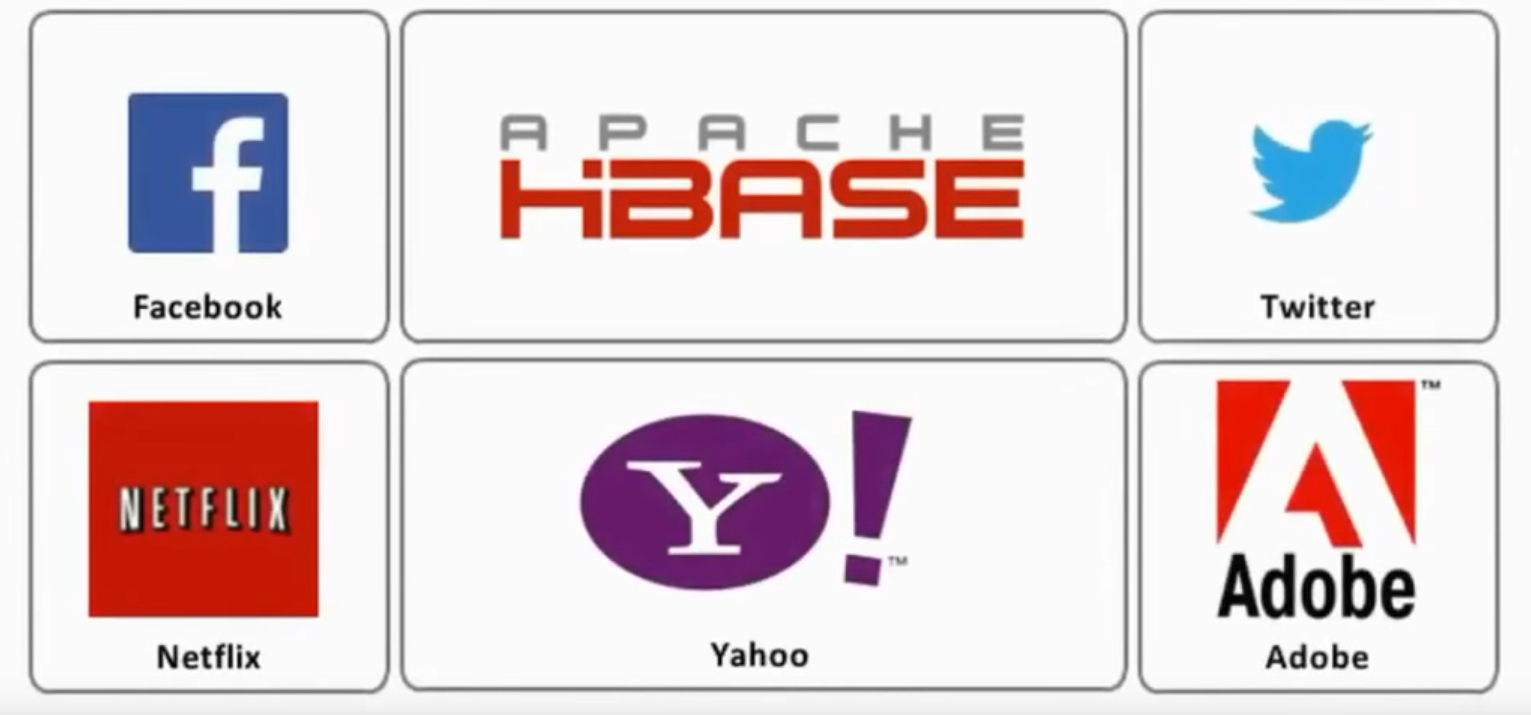
\includegraphics[width=0.7\textwidth]{images/portfolio.png}
  \caption{Portfolio}
  \label{fig:Portfolio}
\end{figure}
Für den Einsatz von HBase gibt es gleich mehrere Gründe:
\begin{itemize}

\item Skalierbarkeit
\item Versionierung
\item Komprimierung
\item Garbage Collection
\item speicherbasierte Tabellen
\item Durch write-ahead-Logging und eine verteilte Konfiguration kann sich Hbase schnell von Serverausfällen erholen
\item Bietet geringe Latenz bei Zugriff auf kleine Teil-Datenmengen 
\item Bietet ein flexibles Datenmodel
\end{itemize}

\subsection{Abgrenzung}
\subsubsection{Hbase im Vergleich zu einem relationalen Datenbank-Managementsystem}
HBase speichert die teils unvollständigen Daten in Spalten ab im Vergleich zu vollständigen Reiheneinträgen in einem RDBMS. Dies ist notwendig da große Datenmengen den Anforderungen auf Vollständigkeit, wie sie ein RDBMS erfordert, oftmals nicht gerecht werden.  
\subsubsection{Hbase im Vergleich zu HDFS}


\subsection{Datenmodell}


\subsection{Tabellenformat}
HBase speichert die Daten, ähnlich wie eine relationale Datenbank in Tabellen. Jedoch bestehen diese aus Reihenschlüsseln und Spaltenfamilien. Es gibt zwei Arten von Tabellen: Die Benutzer-Tabellen und die System-Tabellen.
Die Systemtabellen werden für das Verrwalten von ACLs) verwendet, Meta-Daten für die Tabellen und Regionen und Namensräumen. Die Benutzer-Tabellen werden für die Verwaltung des Milion-Song-Dataset verwendet.

\subsubsection{Regionen}
Eine Tabelle besteht aus Spalten und Reihen. Für die Skalierung  und den randomisierten Zugriff, teilt HBase die Tabelle in Regionen auf. Jede Region wird einem RegionServer zugeordnet. Der HBase LoadBalancer sorgt dafür, dass die Last, also die Regionen auf alle Regionserver gleich verteilt werden. Jede Region wird durch einen StartSchlüssel und einen Endschlüssel begrenzt. Diese Informationen lassen sich in den System-Tabellen wiederfinden. Regionen können geteilt werden, wenn sie zu groß werden oder zusammengelegt werden, wenn die zu klein sind.

\subsubsection{Spaltenfamilien}
Die Vorgabe ist, dass Daten mit gleichen Zugriffs-Querries und dem selben Format in eine Spaltenfamilie gefasst werden sollten. Wenn wir beispielsweise zu zu allen Songs des One-Million-Song-DataSets die Cover der CD's hinterlegt hätten, könnten die Bilder in einer Spaltenfamilie und die textuellen Informationen zu den Songs in einer anderen Spaltenfamilie hintelgt werden. So könnte die Spaltenfamilie mit den textuellen Informationen komprimiert werden. Oder wenn bestimmte Daten nur gelesen werden und andere meistens geschrieben werden, sollte über eine zweite Spaltenfamilie nachgedacht werden. Es gibt keine Grenze nach oben für die Spaltenfamilien innerhalb einer Tabelle, jedoch leidet die Performanz. Der Memorystore wird belastet und generiert viele kleine Dateien.

\subsubsection{Stores}
Es gibt einen Store pro Spaltenfamilie. EIn Store gruppiert den memstore und 0-x mem store files (HFiles). Diese Datei beinhaltet alle Informationen, de in die Tabelle hereingeschrieben und herausgelesen werden.

\subsubsection{Hfiles}
HFiles werden erzeugt, wenn die MemStores voll sind und werden im HDFS abgespeichert, um von der Hadoop-Persistierung und Replikation zu profitieren. HFiles bestehen aus Blöcken. Ein Block hat eine Größe zwischen 8KB und 1 MB. Die Blockgröße kann konfigurtiert werden.  DIe DefaultGröße liegt bei 64KB. Es gibt viel Blcoktypen die innerhalb eines HFiles vorkommmen können: Der Datenblock enhält sowohl die Daten als auch ide put und delete Markierungen. Indexblocks ermöglichen das schnelle Auffinden einer Reihe innerhalb eines HFiles. Bloom-Filter-Blocks werden für das Überspringen von  bestimmten Parse-Vorgängen gentzt, damit der angefragte Schlüssel schneller gefunden werden kann. Trailer Blocks enthalten die HFile-Version.

\subsection{Interne Tabellenoperationen}
Die große Stäke von HBase ist es Daten zu größeren Dateien zusammenzufassen und Tabellen auf mehrere Server zu verteilen. Hierzu verwendet HBase drei verschiedene Mechanismen.

\subsubsection{Verdichtung}
HBase speichert alle Operationen im MemStore ab. Falls dieser voll ist werden die HFiles in das Filesystem geschrieben. Um zu vermeiden, dass viele kleine HFiles entstehen, verdichtet HBase sie zu größeren Dateien. Beim Löschen von Zellen setzt HBase einen Marker, der bei der Verdichtung überprüft wird. Alle Dateien mit dem gleichen Schlüssel, aber einem älteren Zeitstempel werden so gelöscht. In einer weiteren Stufe der Verdichtung können alle Marker gelöscht werden. Eine solche Verdichtung kann manuell für eine spezifische Region oder Tabelle angestoßen werden. Außerdem werden standardmäßig wöchentlich solche Verdichtungen von HBase selbst ausgeführt.

\subsubsection{Teilung}
Das Gegenteil der Verdichtungen ist die Teilung (Split), auch Auto-Sharding genannt. Wenn eine Region eine Größe von 10GB erreicht, führt HBase eine Teilung durch und es entstehen zwei neue Regionen. Hierbei ist zu beachten, dass Teilungen immer spaltenfamileienübergreifend stattfinden (siehe Abbildung).

\begin{figure}[htbp] 
  \centering
     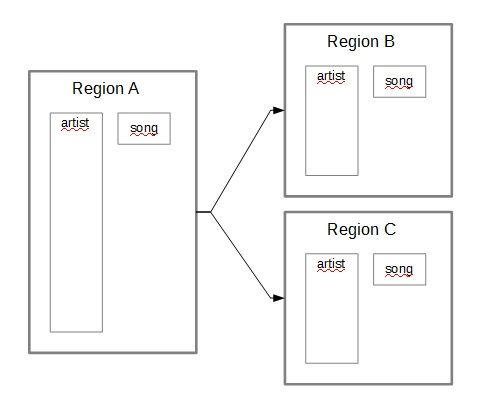
\includegraphics[width=0.7\textwidth]{images/split.jpg}
  \caption{Zwei Spaltenfamilien nach vor und nach der Teilung}
  \label{fig:Teilung}
\end{figure}


\subsubsection{Verteilung der Last}
Da Regionen geteilt und verdichtet werden, neue Server hinzukommen oder herunterfahren ist eine Balancierung der Last notwendig. HBase führt alle fünf Minuten einen LoadBalancer aus der algorithmisch sicherstellt, das alle RegionServer eine ähnliche Anzahl an Regionen bedienen. 

\subsection{Master-Slave-System}
Habse besitzt zwei Rollen: den HBase Master Server und die RegionServer.

\subsubsection{Master Server}
Der Master Server ist verantwortlich für die Zuweisung der regionen an die RegionServer, die Verteilung der Last (Link), den Neustart der RegionServer, die Teilung (Link) und das Überwachen der RegionServer. Es ist möglich mehrere Master in einem Cluster zu betrieben, wobei aber nur einer aktiv sein kann. Da der Master nur verwaltende Funktionen inne hält, kann ein Cluster auch ohne Master Server arbeiten, solange kein RegionServer ausfällt. Spätestens dann muss der Master Server eingreifen und die Regionen neu zuweisen.

\subsubsection{RegionServer}


Hbase benütigt kein Schema und unterstützt ein flexibles Datenmodell, indem ein Hinzufügen einer neuen Spalte jederzeit mögich ist. Daten werden in Tabellen gespeichert.

\subsection{Zugriff auf HBase}
\begin{itemize}

\item JAVA
\item REST
\item Avro
\item Thrift
\end{itemize}



Des weiteren erinnert HBase an eine relationale Datenbank, da sie ihre Daten in Tabellen speichert, die Zellen enthalten. Jedoch verhalten sich die Tabellen nicht wie Relationen und Zeilen nicht wie Datensätze in relationalen Datenbanken. Auch sind die Spalten nicht durch ein Schema definiert.

Da HDFS ein Filesystem ist, fehlt ihm die zufällige Lese-und Schreibfähigkeit. Eine mögliche Lösung dafür ist HBase. Es wird innerhalb des Hadoop-Clusters betrieben und stellt in Echtzeit Lese- und Schreibzugriff zu den Daten her. HBase ist besonders wertvoll, wenn es um die Verarbeitung von sehr großen Datenmengen geht. Aus diesem Grund wird es auch oftmals als Logging- und Suchsystem in großen Unternehmen eingesetzt.





\subsection{Installation und Konfiguration von HBase}